\documentclass[noinstructornotes]{ximera}
%handout:  for handout version with no solutions or instructor notes
%handout,instructornotes:  for instructor version with just problems and notes, no solutions
%noinstructornotes:  shows only problem and solutions

%% handout
%% space
%% newpage
%% numbers
%% nooutcomes

%I added the commands here so that I would't have to keep looking them up
%\newcommand{\RR}{\mathbb R}
%\renewcommand{\d}{\,d}
%\newcommand{\dd}[2][]{\frac{d #1}{d #2}}
%\renewcommand{\l}{\ell}
%\newcommand{\ddx}{\frac{d}{dx}}
%\everymath{\displaystyle}
%\newcommand{\dfn}{\textbf}
%\newcommand{\eval}[1]{\bigg[ #1 \bigg]}

%\begin{image}
%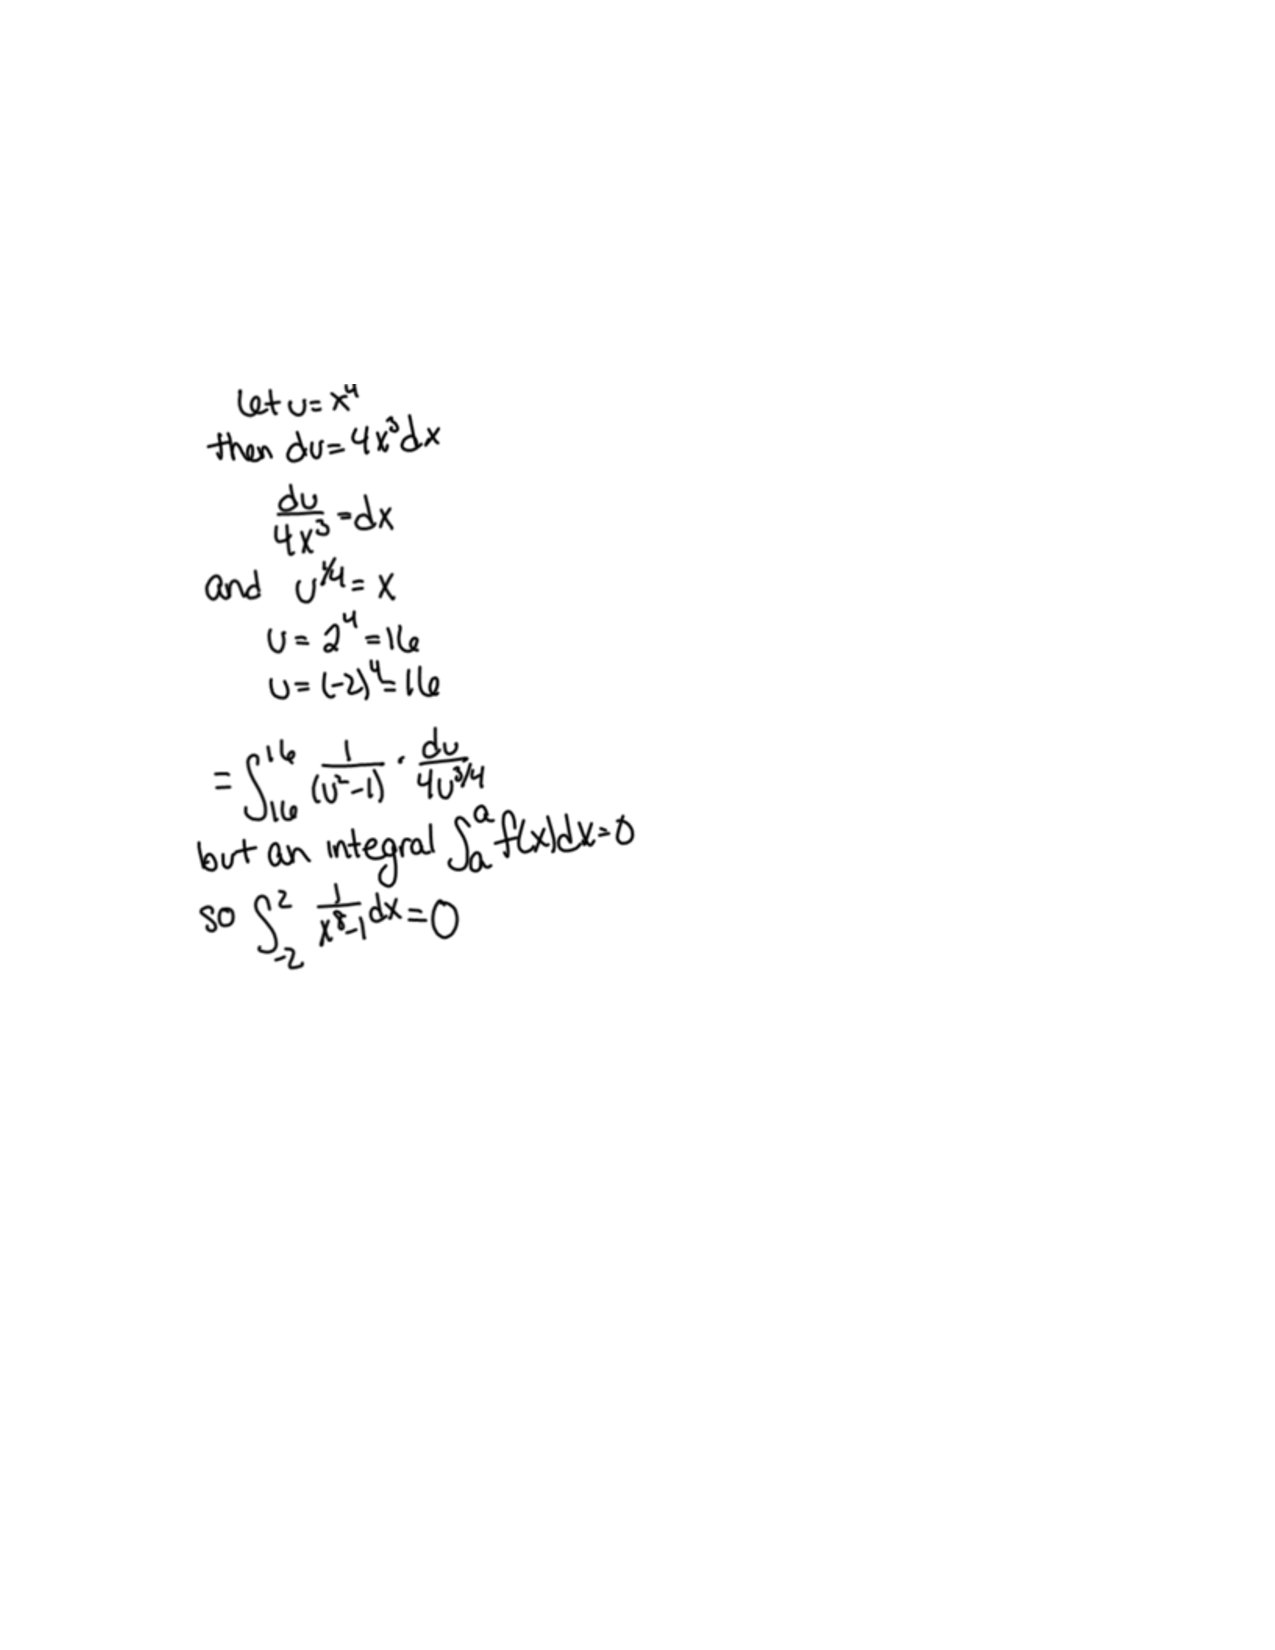
\includegraphics[trim= 170 420 250 180]{Figure1.pdf}
%\end{image}

%add a ``.'' below when used in a specific directory.
\newcommand{\RR}{\mathbb R}
\renewcommand{\d}{\,d}
\newcommand{\dd}[2][]{\frac{d #1}{d #2}}
\renewcommand{\l}{\ell}
\newcommand{\ddx}{\frac{d}{dx}}
\newcommand{\dfn}{\textbf}
\newcommand{\eval}[1]{\bigg[ #1 \bigg]}

\usepackage{multicol}

\renewenvironment{freeResponse}{
\ifhandout\setbox0\vbox\bgroup\else
\begin{trivlist}\item[\hskip \labelsep\bfseries Solution:\hspace{2ex}]
\fi}
{\ifhandout\egroup\else
\end{trivlist}
\fi} %% we can turn off input when making a master document


\title{Section 9.1: An Overview of Sequences and Series}  

\begin{document}
\begin{abstract}		\end{abstract}
\maketitle




\section{Warm up:}

	For each of the following sequences, list the first four terms (start each with $n=1$).
	\begin{enumerate}
	\item 	$a_{n+1} = \frac{1}{2} \left( a_n + \frac{2}{a_n} \right), \; a_1 = 1$.
	\begin{freeResponse}
	\dfn{n=1:}  \; $a_1 = 1$.
	
	\dfn{n=2:}  \; $a_2 = \frac{1}{2} \left( a_1 + \frac{2}{a_1} \right) = \frac{1}{2} \left( 1 + \frac{2}{1} \right) = \frac{3}{2}$.
	
	\dfn{n=3:}  \; $a_3 = \frac{1}{2} \left( a_2 + \frac{2}{a_2} \right) = \frac{1}{2} \left( \frac{3}{2} + \frac{2}{\frac{3}{2}} \right) = \frac{17}{12}$.
	
	\dfn{n=4:}  \; $a_4 = \frac{1}{2} \left( a_3 + \frac{2}{a_3} \right) = \frac{1}{2} \left( \frac{17}{12} + \frac{2}{\frac{17}{12}} \right) = \frac{577}{408}.$
	\end{freeResponse}
	
	
	
	\item 	$a_n = \frac{1 \cdot 3 \cdot 5 \hdots (2n-1)}{(2n)! \cdot 2n!}, \; \text{ Recall that }n! = 1 \cdot 2 \cdot 3 \cdot 4 \hdots (n-1) \cdot n$.
	\begin{freeResponse}
	\dfn{n=1:}  \; $a_1 = \frac{1}{2! 2!} = \frac{1}{4}$.
	
	\dfn{n=2:}  \; $a_2 = \frac{1 \cdot 3}{(2 \cdot 2)! \cdot 2 \cdot 2!} = \frac{3}{96} = \frac{1}{32}$.
	
	\dfn{n=3:}  \; $a_3 = \frac{1 \cdot 3 \cdot 5}{6! \cdot 2 \cdot 3!}$.
	
	\dfn{n=4:}  \; $a_4 = \frac{1 \cdot 3 \cdot 5 \cdot 7}{8! \cdot 2 \cdot 4!}$.
	\end{freeResponse}
	\end{enumerate}
	
\begin{instructorNotes}
For this handout, the problems are rather short. I suggest having all groups do each part.
\end{instructorNotes}








\section{Group work:}










%problem 1
\begin{problem}
Give an explicit formula for each of the following sequences:
	\begin{enumerate}
	\item 	$\frac{2}{3}, \frac{-2}{7}, \frac{2}{11}, \frac{-2}{15}, \hdots$
	\begin{freeResponse}
	$a_n = \frac{(-1)^{n+1} \cdot 2}{-1 + 4n}$, starting at $n=1$.
	\end{freeResponse}
	
	
	
	\item 	$-2, 6,-24,120,-720, \hdots$
	\begin{freeResponse}
	$a_n = (-1)^n (n+1)!$, starting at $n=1$.
	\end{freeResponse}
	
	
	
%	\item 	$2,8,26,80,242,\hdots$
%	\begin{freeResponse}
%	$a_n = 3^n - 1$, starting at $n=1$.
%	\end{freeResponse}
	\end{enumerate}
		
\end{problem}

\begin{instructorNotes}

\end{instructorNotes}







%problem 2
\begin{problem}
For the sequence $a_k = (2-k)^k$
	\begin{enumerate}
	\item 	calculate and list $a_0$, $a_1$, $a_2$, $a_3$, and $a_4$.
	\begin{freeResponse}
	$a_0 = (2-0)^0 = 1$.  \\
	$a_1 = (2-1)^1 = 1$.  \\
	$a_2 = (2-2)^2 = 0$.  \\
	$a_3 = (2-3)^3 = -1$.  \\
	$a_4 = (2-4)^4 = 16$.  
	\end{freeResponse}
	
	
	
	\item 	Starting with $k=0$, calculate and list $S_0 = \sum_{k=0}^0 a_k$, $S_1 = \sum_{k=0}^1 a_k$, 
	$S_2 = \sum_{k=0}^2 a_k$, $S_3 = \sum_{k=0}^3 a_k$, and $S_4 = \sum_{k=0}^4 a_k$.  
	Write $S_n$ in summation form and write $S_\infty$ in summation form.
	\begin{freeResponse} We have \\
	$S_0 = \sum_{k=0}^0 a_k = a_0 = (2-0)^0 = 1$.  \\
	$S_1 = \sum_{k=0}^1 a_k = a_0 + a_1 = (2-0)^0 + (2-1)^1 = 1+1 = 2$.  \\
	$S_2 = \sum_{k=0}^2 a_k = a_0 + a_1 + a_2 = S_1+a_2 = 2 + (2-2)^2 = 2$.  \\
	$S_3 = \sum_{k=0}^3 a_k = a_0 + a_1 + a_2 + a_3 = S_2 + a_3 = 2+ (2-3)^3 = 1$.  \\
	$S_4 = \sum_{k=0}^4 a_k = a_0 + a_1 + a_2 + a_3 + a_4 = S_3 + (2-4)^4 = 1+16 = 17$.  \\
	$S_n = \sum_{k=0}^n (2-k)^k =  (2-0)^0 +(2-1)^1 + (2-2)^2 + (2-3)^3 + ... +  (2-n)^n  $  \\
	$S_\infty = \lim_{n \to \infty}\sum_{k=0}^n a_k = \lim_{n \to \infty} \sum_{k=0}^n (2-k)^k = \\   \lim_{n \to \infty} [(2-0)^0 +(2-1)^1 + (2-2)^2 + (2-3)^3 + ... +  (2-n)^n]  $.  
	\end{freeResponse}
	\end{enumerate}
	
\end{problem}

\begin{instructorNotes}

\end{instructorNotes}







%%problem 3
%\begin{problem}
%For each of the following, write the series in the form $\sum_{k=0}^\infty a_k$.
%	\begin{enumerate}
%	\item 	$0.2 + 0.06 + 0.018 + 0.0054 + \hdots$
%	\begin{freeResponse}
%	$\sum_{k=0}^\infty 0.2 \left(\frac{3}{10} \right)^k$.
%	\end{freeResponse}
%	
%	
%	
%	\item 	$\frac{1}{2} + \frac{1}{3^2} - \frac{1}{3} - \frac{1}{4^2} + \frac{1}{4} + \frac{1}{5^2} - \frac{1}{5} - \frac{1}{6^2} \hdots$
%	\begin{freeResponse}
%	$\sum_{k=1}^\infty \left[ (-1)^k \left( \frac{1}{k+2} + \frac{1}{(k+3)^2} \right) \right] $.
%	\end{freeResponse}
%	\end{enumerate}
%
%\end{problem}
%
%\begin{instructorNotes}
%
%\end{instructorNotes}







%problem 4
\begin{problem}
Reindex the series
	\[
	\sum_{k=0}^\infty \frac{5}{(k+2)(k+1)}
	\]
in the form $\sum_{k=1}^\infty a_k$ and $\sum_{k=-4}^\infty c_k$.
	\begin{freeResponse}
	For the first series, we let $i = k+1$.
	Then $k = i-1$ and, when $k=0$, $i = 1$.
	So we have that
		\begin{align*}
		\sum_{k=0}^\infty \frac{5}{(k+2)(k+1)}
		&= \sum_{i=1}^\infty \frac{5}{(i-1+2)(i-1+1)}  \\
		&= \sum_{i=1}^\infty \frac{5}{i(i+1)}  \\
		&= \sum_{k=1}^\infty \frac{5}{k(k+1)}.  	\qquad	{\color{red}\text{Resubstituting k=i.}}
		\end{align*}
		
	For the second series, we let $i=k-4$.  
	Then $k=i+4$ and, when $k=0$, $i = -4$.  
	So we have that
		\begin{align*}
		\sum_{k=0}^\infty \frac{5}{(k+2)(k+1)}
		&= \sum_{i=-4}^\infty \frac{5}{(i+4+2)(i+4+1)}  \\
		&= \sum_{i=-4}^\infty \frac{5}{(i+5)(i+6)}  \\
		&= \sum_{k=-4}^\infty \frac{5}{(k+5)(k+6)}.  	\qquad	{\color{red}\text{Resubstituting k=i.}}
		\end{align*}
	\end{freeResponse}

\end{problem}

\begin{instructorNotes}

\end{instructorNotes}







%problem 5
\begin{problem}
If $\sum_{k=0}^\infty a_k = 6$ and $a_n = \frac{3}{2^n}$, what is $\sum_{k=4}^\infty a_k$?
	\begin{freeResponse}
		\begin{align*}
		6 &= \sum_{k=0}^\infty a_k  \\
		&= a_0 + a_1 + a_2 + a_3 + \sum_{k=4}^\infty a_k  \\
		&= \frac{3}{1} + \frac{3}{2} + \frac{3}{4} + \frac{3}{8} + \sum_{k=4}^\infty a_k  \\
		&= \frac{45}{8} + \sum_{k=4}^\infty a_k.
		\end{align*}
	Thus,
		\[
		\sum_{k=4}^\infty a_k = 6 - \frac{45}{8} = \frac{3}{8}.
		\]
	\end{freeResponse}

\end{problem}

\begin{instructorNotes}

\end{instructorNotes}
















	
	
	
	
	
	
	
	
	

	










								
				
				
	














\end{document} 


















